\chapter[Introduction]{Introduction}
\label{ch: Intro}

During the last two decades, the world has seen an increasing participation of renewable sources in power generation, leaded mainly by wind and solar energy. These technologies provide an alternative to sources based on fossil fuel, such as oil, gas and coal, lowering pollution levels and reducing greenhouse gas emissions. On the other hand, the power output from these sources strongly relies on weather conditions and cannot be fully controlled.

This increase is seen worldwide, as part of policies to reduce the human impact on climate and the environment. This `renewable wave' is leaded mainly by European countries, specially in the European Union (EU), United States (US) and China. In particular, the EU has set in 2010 a strategy plan to reduce its greenhouse emissions by at least 20\% compared to 1990 levels and increase the share of renewable sources to at least 20\% by 2020 \cite{Europe2020}.

Brazil does not lag far behind the EU regarding renewable sources policies. In 2002, the country passed a bill that, among other actions, creates the Program of Incentive to Alternative Electric Energy Sources (PROINFA). This program aims to increase the share of wind, solar, small hydro and biomass energy production. The final goal is to have these energy sources corresponding to 10\% of Brazil's annual energy consumption by 2024 \cite{Brazil2002}.

\section{Wind Energy}

Those policies promoted the increase of wind energy participation, reaching a scenario where it is one of the main energy sources of some countries, such as Denmark and Ireland. In the EU, wind energy alone generated 417 TWh in 2019, covering 15\% of the electricity demand, a share 1\% higher than 2018, with wind turbine generators (WTGs) installed both onshore (within the countries) and offshore (in the ocean). Among the EU countries, Denmark leads in this sector, with 48\% of its demand supplied by wind power plants (WPPs), followed by Ireland (33\%), Portugal (27\%) and Germany (26\%). The total installed capacity across the 28 EU countries (UK included) is 192 GW, with Germany in first position, with a total installed capacity of 61 GW, followed by Spain and the United Kingdom (UK), with 26 and 24 GW installed, respectively \cite{WindEurope2020}. Figure \ref{fig: EUrank} displays the detailed percentage of electricity demand covered by wind in the EU.

\begin{figure}[h]
	\caption{Share of electricity demand in the EU covered by wind energy during 2019}
	\begin{center}
		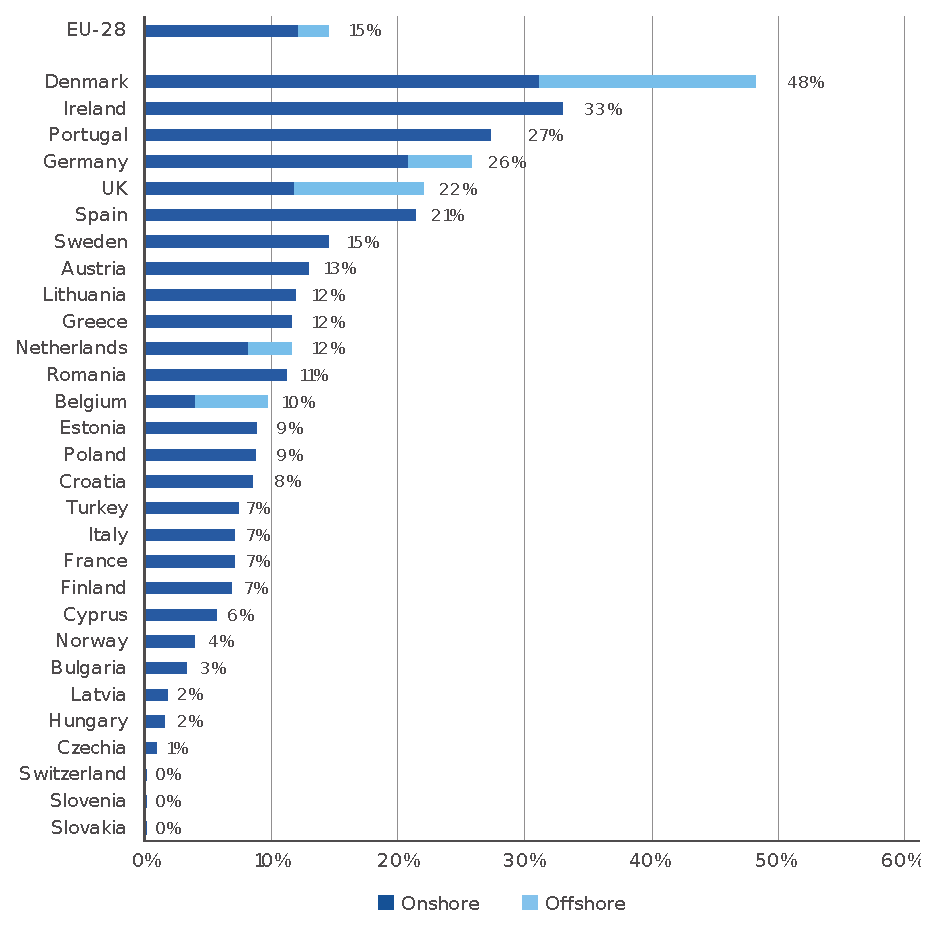
\includegraphics[scale=0.65]{Images/EUrank2019.eps}
	\end{center}
	\label{fig: EUrank}
	\legend{Source: Wind Europe, 2020}
\end{figure}

In Brazil, wind energy contributed to the electricity matrix with 48.5 TWh during 2018, resulting in a participation share of 8.1\%. For comparison, Itaipu, the largest power plant in Brazil, has produced 96.5 TWh during the same period. But, while other sources, such as gas and coal, had their share lowered, wind energy had the highest increase among sources comparing to 2017, increasing its contribution by 14.4\% \cite{EPE2019}.

Regarding the installed capacity, wind power plants appear in \nth{2} place, with 15.5 GW installed, only behind hydro power plants \cite{ABEEolica2020}, as shown in Figure \ref{fig: BRshare}. However, there is still plenty of energy yield for this source to be explored. In \cite{Atlas2001} is shown that Brazil has potential to generate 272.2 TWh per year, with an installed capacity of 143.5 GW. The Northeast Region has the higher potential, with an annual energy yield of 144.3 TWh and potential to host up to 75.0 GW. Also, the wind regime in the Northeast Region is complimentary to the water regime of the main river responsible to power generation in the region, as presented by Figure \ref{fig: WindWater}. This characteristic would help controlling reservoir water level during dry season, an important resource not only for power generation, but also irrigation of crops and water supply \cite{ANEEL2005}.

\begin{figure}[ht]
	\caption{Electricity generation in Brazil by source during 2019}
	\begin{center}
		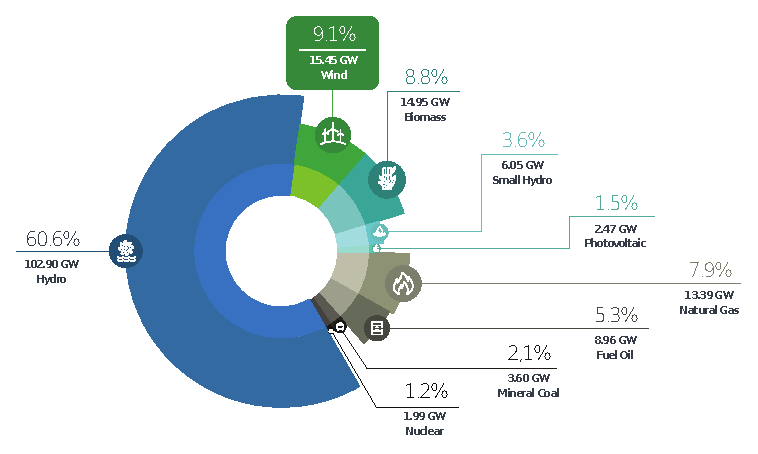
\includegraphics[scale=0.8]{Images/BRshare20.eps}
	\end{center}
	\label{fig: BRshare}
	\legend{Source: ABEE\'olica, 2019}
\end{figure}

\begin{figure}[hb]
	\caption{Wind and water regime in the Brazilian Northeast Region}
	\begin{center}
		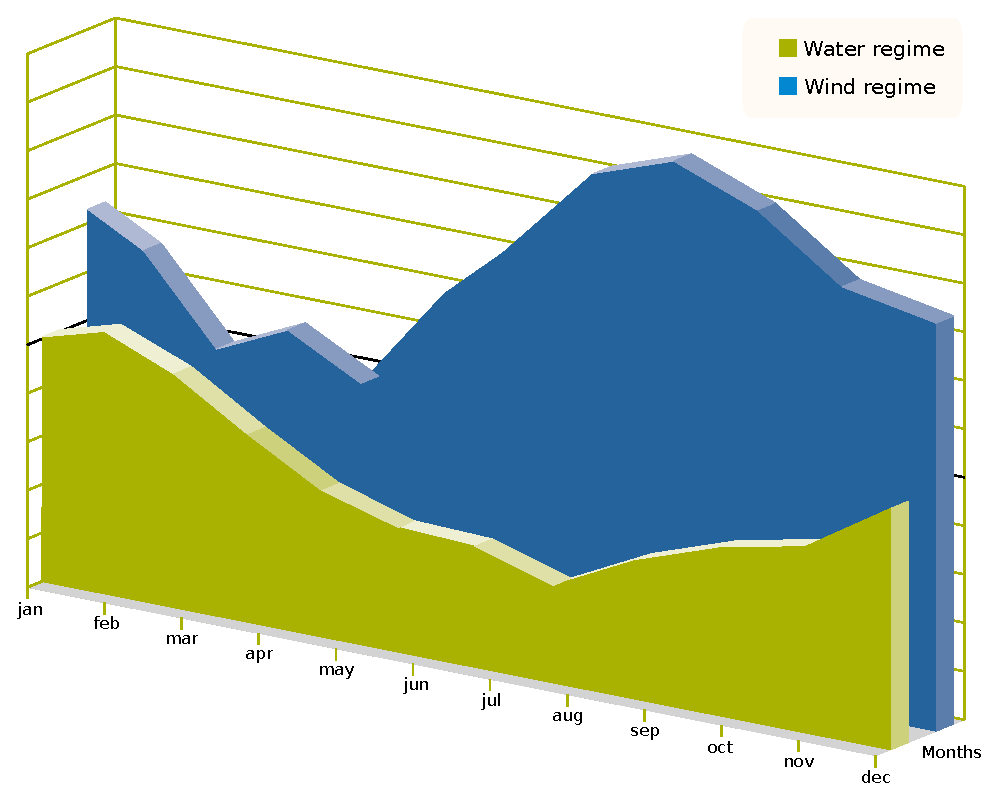
\includegraphics[scale=0.5]{Images/WindWater.eps}
	\end{center}
	\label{fig: WindWater}
	\legend{Source: ANEEL, 2005}
\end{figure}

Therefore, it is expected that wind energy will increase its participation in electricity generation in the near future. However, some aspects of the wind energy must be considered prior to the implementation of wind power plants on large scale.

The main difficulties are due to the nature of the energy source and characteristics of the generator. The wind regime is not constant and evenly distributed across the country, depending on the region geography and vegetation. This results in a energy source that is not entirely reliable and concentrated on a certain area. Wind turbine generators are usually partially or entirely decoupled from the grid via power electronic converters, resulting in machines with low inertia. Thus, the system may experience stability problems during transients due to the high penetration of these machines \cite{Xiong2019}.

In order to maintain the electrical power system reliable, studies simulating various conditions must be performed beforehand, so the operators can be prepared for different fault scenarios. Therefore, robust mathematical models, capable of adequately simulate the behaviour of every component on the grid, are vital to these studies. Otherwise, operators will not be able to solve the fault problem or even provide a solution that will aggravate the fault.

\section{Difficulties in Representing Wind Power Plants}

With a growing share of energy covered by wind, system operators must consider how wind turbines affect the system stability during faults and maneuvers. To reach this goal, mathematical models capable of describing the behaviour of these machines are crucial. 

Obtaining these models, on the other hand, is not an easy task. Due to confidentiality, most manufacturers provide little or no information about the functioning of their wind turbine generators. In addition, there is a great amount of WTGs available, with different manufacturers, technologies, sizes and characteristics. Thus, a model that well describes a particular machine will not necessarily work for others.

Modelling entire wind power plants is even harder, since these facilities contain a large variety of WTGs spread over a wide area. Besides, line impedance of each generator is different, since their distances to the substation is not the same, as depicted in Figure \ref{fig: WPP}. Hence, having one model for every wind turbine within a power plant would result in a mathematical model with high computational cost and extremely complex \cite{Erlich2012}.

\begin{figure}[h]
	\caption{Example of Wind Power Plant}
	\begin{center}
		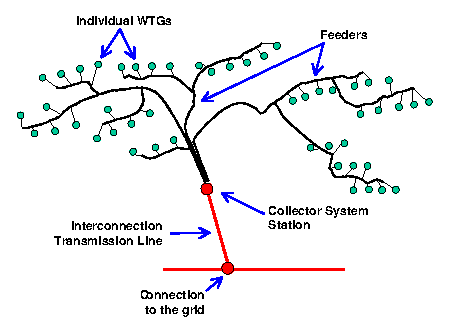
\includegraphics[scale=1.25]{Images/WPP.eps}
	\end{center}
	\label{fig: WPP}
	\legend{Source: Adapted from \cite{Muljadi2008}}
\end{figure}

In order to avoid using such complex models, many studies addressed the application of generic equivalent models to simulate the behaviour of WPPs. In particular, \cite{Ellis2011} shows that most wind power plants can be represented by a single-machine equivalent model. The benefits of using such equivalent model include reduction on model complexity and the fact it can be adjusted to match any given wind power plant. On the downside, these models cannot reproduce how particularities of each generator, such as wind speed and low voltage ride through capability, affects the WPP behaviour.

\section{Research Goals}

The main goal of this research is to develop a software for parameter estimation of nonlinear model and apply it to a wind power plant equivalent model used in transient stability studies. In order to achieve this goal, a hybrid estimation approach was applied combining two methods: Mean-Variance Mapping Optimization, a population-based metaheuristic approach, and Trajectory Sensitivity Method, a nonlinear approach. Also, as a secondary goal, a graphical user interface (GUI) was developed, so other users can easily apply the tool created. This research is a extension of \cite{Cari2015}, that focused on the parameter estimation using only Trajectory Sensitivity Method.

\section{Work Organization}

This section summarizes how the remainder of the text is organized. Chapter \ref{ch: Models} will focus on the generic models for wind turbine generators and power plants and the selected mathematical model for parameter estimation purposes will be presented. The hybrid estimation process proposed and its methods will be subject of chapter \ref{ch: Estimation}. The python package and GUI created in this research will be detailed on chapter \ref{ch: Software}. On chapter \ref{ch: Results}, the results obtained on this research will be discussed. Finally, chapter \ref{ch: Future} covers the future perspectives of this study.